% ============================================================
%  鱼你有图 技术投标文件
%  编译方式: xelatex main.tex
%  文档类: ctexart (中文文章)
% ============================================================
\documentclass[12pt,a4paper]{ctexart}

% ---------- 页面设置 ----------
\usepackage[top=2.5cm,bottom=2.5cm,left=2.8cm,right=2.8cm]{geometry}

% ---------- 字体 ----------
\usepackage{fontspec}
% 不指定系统特有等宽字体，避免跨设备编译失败（Overleaf / Linux 无 Consolas）

% ---------- 图表 ----------
\usepackage{graphicx}
\usepackage{float}
\usepackage{subcaption}
\graphicspath{{figures/}}

% ---------- 表格 ----------
\usepackage{tabularx}
\usepackage{longtable}
\usepackage{booktabs}
\usepackage{array}

% ---------- 代码块 ----------
\usepackage{listings}
\usepackage{xcolor}

\definecolor{codebg}{RGB}{248,248,248}
\definecolor{codeframe}{RGB}{220,220,220}
\definecolor{codekey}{RGB}{0,119,170}
\definecolor{codestr}{RGB}{17,140,55}
\definecolor{codecmt}{RGB}{138,138,138}

\lstset{
  basicstyle          = \small\ttfamily,
  backgroundcolor     = \color{codebg},
  frame               = single,
  framerule           = 0.5pt,
  rulecolor           = \color{codeframe},
  numbers             = left,
  numberstyle         = \tiny\color{gray},
  numbersep           = 6pt,
  breaklines          = true,
  breakatwhitespace   = false,
  showstringspaces    = false,
  captionpos          = t,
  aboveskip           = 8pt,
  belowskip           = 8pt,
  keywordstyle        = \color{codekey}\bfseries,
  stringstyle         = \color{codestr},
  commentstyle        = \color{codecmt}\itshape,
  extendedchars       = true,
  literate            =
    {。}{{。}}1
    {，}{{，}}1
    {；}{{；}}1
    {：}{{：}}1
    {！}{{！}}1
    {？}{{？}}1
    {（}{{（}}1
    {）}{{）}}1
    {「}{{「}}1
    {」}{{」}}1
}

% ---------- 超链接 ----------
\usepackage[colorlinks=true,linkcolor=blue,urlcolor=blue,citecolor=blue]{hyperref}

% ---------- 页眉页脚 ----------
\usepackage{fancyhdr}
\pagestyle{fancy}
\fancyhf{}
\fancyhead[L]{\small 鱼你有图技术投标文件}
\fancyhead[R]{\small 课程实习项目}
\fancyfoot[C]{\thepage}
\renewcommand{\headrulewidth}{0.5pt}

% ---------- 标题格式 ----------
\ctexset{
  section = {
    format    = \Large\bfseries,
    number    = \thesection,
    aftername = \quad,
  },
  subsection = {
    format    = \large\bfseries,
    number    = \thesubsection,
    aftername = \quad,
  },
}

% ---------- 文档标题 ----------
\title{\Huge\bfseries 鱼你有图技术投标文件}
\author{}
\date{}

\begin{document}

% ===== 封面 =====
\begin{titlepage}
  \centering
  \vspace*{3cm}

  {\Huge\bfseries 鱼你有图技术投标文件\par}
  \vspace{0.8cm}
  {\LARGE 面向垂钓场景的 GIS 智能推荐与社交平台\par}

  \vspace{2.5cm}

  \begin{tabular}{rl}
    \textbf{项目类型} & 课程实习项目 \\[6pt]
    \textbf{团队名称} & \quad 占位\_团队名称 \\[6pt]
    \textbf{团队成员} & \quad 占位\_成员一、占位\_成员二、占位\_成员三 \\[6pt]
    \textbf{编写日期} & \quad \today \\[6pt]
    \textbf{版本号}   & \quad v1.0 \\
  \end{tabular}

  \vspace{2cm}
  {\large 武汉大学}
\end{titlepage}

% ===== 目录 =====
\tableofcontents
\newpage

% ===== 正文 =====
\section{项目概述}

\subsection{项目背景}

（待填写：钓鱼爱好者群体的市场规模、用户痛点、现有产品不足。）

\subsection{产品定位}

「鱼你有图」是面向钓鱼爱好者的垂钓 GIS 社交平台，核心目标是帮助用户回答五个问题：
\begin{enumerate}
  \item 去哪钓？
  \item 能不能钓？
  \item 有没有鱼？
  \item 怎么钓？
  \item 和谁一起钓？
\end{enumerate}

\subsection{项目目标}

（待填写：短期 MVP 目标、中期运营目标、长期商业目标。）

\subsection{核心指标}

（待填写：用户量、日活、留存率、推荐准确率等 KPI。）

\section{需求分析}

\subsection{用户角色}

本平台面向四类核心用户角色：

\begin{table}[H]
  \centering
  \caption{用户角色分析}
  \label{tab:user-roles}
  \begin{tabularx}{\textwidth}{p{2.5cm}|p{4.5cm}|p{4.5cm}|p{3.5cm}}
    \toprule
    \textbf{角色} & \textbf{特征} & \textbf{核心需求} & \textbf{平台价值} \\
    \midrule
    钓鱼爱好者（新手） & 对钓鱼感兴趣但经验不足，依赖工具决策 & 可视化地图找点、智能推荐、系统化教程、良好社区氛围 & 降低入门门槛，缩短从“想去钓”到“会钓”的距离 \\
    \hline
    钓鱼爱好者（老手） & 具有稳定出钓频率，关注钓点质量和社群认可 & 钓点质量判断、鱼种/鱼情/钓法信息、装备讨论、战绩展示 & 提供结构化数据沉淀和社群认同感 \\
    \hline
    渔业经营主体 & 钓场、渔庄等，需要展示和获客 & 商户展示、预约转化、赛事组织、用户评价管理 & 精准触达垂钓消费人群 \\
    \hline
    地方监管与服务主体 & 渔政、文旅、农业农村部门 & 禁渔区宣传、文明垂钓引导、违规提醒、产业数据监测 & 提供数字化治理抓手 \\
    \bottomrule
  \end{tabularx}
\end{table}

当前 MVP 阶段优先服务前两类用户（钓鱼爱好者），渔业经营主体和监管服务主体作为后续扩展方向。

\subsection{功能需求}

围绕五个核心用户问题，平台需提供以下功能模块：

\begin{enumerate}
  \item \textbf{地图与 POI 发现}：展示附近钓点、支持关键字搜索与类型筛选（野钓/钓场/海钓/免费/夜钓/路亚）、展示天气摘要、禁钓区与风险图层开关。当前 MVP 阶段基于高德 JS API 实现地图展示，POI 数据以 JSON 集合提供，后续可接入高德 POI 搜索和自建垂钓 POI。
  \item \textbf{POI 详情与推荐}：展示钓点名称、类型、距离、鱼种、收费、设施、规则摘要；基于鱼情分、合规分、距离分、天气适配分、设施便利分、社交热度分计算推荐指数；对禁钓、限钓、极端天气等风险优先提示。
  \item \textbf{出钓记录}：支持鱼获记录、空军记录、探点记录三种类型；自动回填天气、时间、位置；结构化采集鱼种、数量、重量、钓法、饵料、装备等字段；生成可分享的战绩卡片。
  \item \textbf{社区与发布}：支持鱼获流、同城流和话题流；帖子关联出钓记录；内容权限（公开/私密）与位置权限（精确/模糊/隐藏）分离。
  \item \textbf{AI 推荐解释}：后端规则模型完成排序，DeepSeek 将结构化推荐结果解释为自然语言建议，不直接参与排序决策。
  \item \textbf{教程学习}：按新手入门、钓法教程、鱼种攻略、场景攻略等分类组织；教程关联附近练习钓点。
  \item \textbf{个人主页与统计}：展示总出钓、总鱼获、常钓鱼种、高频钓点、偏好时段等统计；当前 MVP 阶段已提供前端展示和后端 profile-summary/report 汇总接口，后续可扩展更完整的月报、年报和会员报告。
\end{enumerate}

\subsection{非功能需求}

\begin{table}[H]
  \centering
  \caption{非功能需求}
  \label{tab:nfr}
  \begin{tabularx}{\textwidth}{p{3cm}|p{6cm}|p{6cm}}
    \toprule
    \textbf{类别} & \textbf{需求描述} & \textbf{MVP 阶段策略} \\
    \midrule
    性能 & 页面首次加载 < 3 秒，地图 POI 渲染流畅 & 前端地图组件动态加载，主 JS 包控制体积 \\
    \hline
    可用性 & 未授权定位时引导授权并提供手动城市选择；API 异常时展示缓存数据和错误提示 & 前端统一错误处理，避免静默降级为假数据 \\
    \hline
    安全性 & API Key 不写入前端代码，用户数据不得通过任意 user\_id 访问 & 第三方 Key 由后端环境变量管理，后续增加基础鉴权 \\
    \hline
    可扩展性 & 前后端分离，接口字段稳定，新增数据集合同步创建 .schema.json & 现有三层架构（路由 → Service → JSON Store）支持逐步演进 \\
    \hline
    兼容性 & 支持微信小程序与 iOS/Android 移动端 & 当前 MVP 先以 Web 移动端完成演示，Uni-app 跨端作为后续方向 \\
    \hline
    数据持久性 & 新增记录和帖子在服务重启后不丢失 & JSON 文件原子读写（临时文件 + 原子替换） \\
    \bottomrule
  \end{tabularx}
\end{table}

\subsection{竞品分析}

当前垂钓相关产品呈现“多而分散”的格局，用户完成一次出钓决策通常需要切换多个平台：

\begin{table}[H]
  \centering
  \caption{竞品格局分析}
  \label{tab:competitors}
  \begin{tabularx}{\textwidth}{p{2.5cm}|p{4cm}|p{4cm}|p{4.5cm}}
    \toprule
    \textbf{类型} & \textbf{代表产品} & \textbf{优势} & \textbf{不足} \\
    \midrule
    传统地图平台 & 高德地图、百度地图 & 底图能力强、POI 检索成熟、导航体验好 & 缺乏垂钓语义层，无法回答“能不能钓、有没有鱼” \\
    \hline
    垂直钓鱼社区 & 钓鱼人、钓鱼之家 & 社区氛围强、内容深度好、用户信任度高 & 地图表达弱、政策整合不足、数据标准化程度低 \\
    \hline
    泛内容平台 & 抖音、小红书、B站 & 流量巨大、内容分发能力强、适合破圈传播 & 地点可信度弱、信息结构化程度低、难以沉淀为空间数据资产 \\
    \hline
    工具类平台 & 墨迹天气、两步路、中国海洋预报 & 单点问题解决能力强、用户理解成本低 & 无法覆盖完整出钓链路（找点→判断→记录→分享→复盘） \\
    \bottomrule
  \end{tabularx}
\end{table}

「鱼你有图」的定位不是再造一个地图或论坛，而是在成熟地图底图之上叠加垂钓专题 POI、禁钓规则、鱼情数据和钓友内容，形成差异化的垂钓 GIS 应用层；同时把泛内容平台作为内容引流阵地，承接用户从“看到鱼获”到“查询钓点、判断规则、规划出行、记录鱼获”的后续决策链路。

\section{总体方案}

\subsection{方案架构概述}

本方案采用\textbf{前后端分离}的 Web 应用架构，前端负责页面渲染与用户交互，后端负责业务逻辑与数据持久化，前后端通过 RESTful API 通信。

整体技术路线：

\begin{itemize}
  \item \textbf{前端}：Vue 3 + Vite + Element Plus + 高德 JS API 2.0，实现移动端优先的单页应用
  \item \textbf{后端}：FastAPI（Python 3.11）+ Pydantic 2，提供统一 `/api` 入口
  \item \textbf{数据层}：根目录 `data/` 下 JSON 文件模拟 NoSQL 集合，每个集合配 `.schema.json` 描述文件，写入采用临时文件 + 原子替换策略
  \item \textbf{第三方服务}：高德 Web 服务（POI 搜索、天气查询）和 DeepSeek API（智能建议生成）均由后端代理调用，API Key 通过环境变量管理
  \item \textbf{开发环境}：前端 `npm run dev`（Vite 开发服务器，端口 5173，代理 `/api` 到后端 8000）；后端 `uvicorn --reload`（端口 8000）；Python 依赖通过 conda 环境 `fish` + `requirements.txt` 管理
\end{itemize}

\subsection{核心设计理念}

本方案以「\textbf{先记录，再连接，后服务}」为核心产品链路：

\begin{enumerate}
  \item \textbf{先记录}：开竿计时 → 真实鱼获录入（鱼种、条数、重量、钓法、饵料）→ 形成个人钓鱼档案。MVP 阶段已实现记录 CRUD 接口、收竿汇总弹窗和 JSON 文件持久化，确保数据在服务重启后不丢失。
  \item \textbf{再连接}：记录关联帖子 → 位置脱敏（精确/模糊/隐藏三级）→ 社区互动。当前阶段帖子可从出钓记录一键生成，社区频道支持按内容类型筛选；后续可扩展评论、点赞、收藏的后端持久化。
  \item \textbf{后服务}：报告识别短板 → 推荐教程/活动/装备 → 产生服务收入。MVP 阶段已实现基于前端的生涯汇总统计（总鱼获、常钓鱼种、高频钓点、偏好时段等），后续可扩展为后端计算的月报/年报和个性化推荐。
\end{enumerate}

\subsection{三层架构设计}

后端采用经典的三层架构，职责清晰、便于测试和扩展：

\begin{table}[H]
  \centering
  \caption{后端三层架构}
  \label{tab:backend-layers}
  \begin{tabularx}{\textwidth}{p{3cm}|p{6cm}|p{5cm}}
    \toprule
    \textbf{层次} & \textbf{职责} & \textbf{MVP 阶段实现} \\
    \midrule
    API 路由层 (\texttt{app/api/}) & 接收 HTTP 请求、参数校验、调用 Service、返回响应 & routes\_poi、routes\_posts、routes\_records、routes\_recommend、routes\_weather、routes\_ai \\
    \hline
    业务服务层 (\texttt{app/services/}) & 业务逻辑聚合、推荐计算、第三方服务封装 & poi\_service、record\_service、post\_service、recommend\_service \\
    \hline
    数据持久层 (\texttt{backend/app/data/json\_store.py}) & JSON 集合的加载、保存、原子更新 & load\_collection、save\_collection、update\_collection（临时文件 + 原子替换） \\
    \bottomrule
  \end{tabularx}
\end{table}

\subsection{关键指标响应}

针对课程实习技术评分表（50 分制，7 个维度），本方案的响应策略如下：

\begin{table}[H]
  \centering
  \caption{关键评分指标响应摘要}
  \label{tab:score-response}
  \begin{tabularx}{\textwidth}{p{0.6cm}|p{3.5cm}|p{4.5cm}|p{5.5cm}}
    \toprule
    \textbf{序号} & \textbf{评分项} & \textbf{分值} & \textbf{方案响应要点} \\
    \midrule
    1 & 项目定位与需求响应 & 6 & 明确五个核心用户问题，划定 MVP 边界，不将非 MVP 内容作为当前交付 \\
    \hline
    2 & 核心功能完成度 & 15 & 跑通“地图找点→详情→推荐→发布→社区”主流程，各页面可演示且数据联动 \\
    \hline
    3 & 技术架构与接口设计 & 8 & 前后端边界清晰，接口字段稳定，第三方 Key 由后端环境变量管理 \\
    \hline
    4 & 推荐模型与AI解释 & 7 & 规则模型六维评分 + 硬性拦截，AI 只做解释不改排序 \\
    \hline
    5 & 数据结构与数据可用性 & 5 & 核心模型（FishingPOI、FishingRecord、CatchPost 等）字段完整，JSON 集合配 schema 文件 \\
    \hline
    6 & 界面交互与演示体验 & 5 & 地图即首页，POI 卡片→详情→发布→社区路径顺畅，视觉风格统一 \\
    \hline
    7 & 文档规范与团队协作 & 4 & 技术投标文件、产品/功能/开发设计书齐备，编号统一，内容与实现一致 \\
    \bottomrule
  \end{tabularx}
\end{table}

\section{系统架构设计}

\subsection{整体架构图}

（待放置系统架构图。）

\begin{figure}[H]
  \centering
  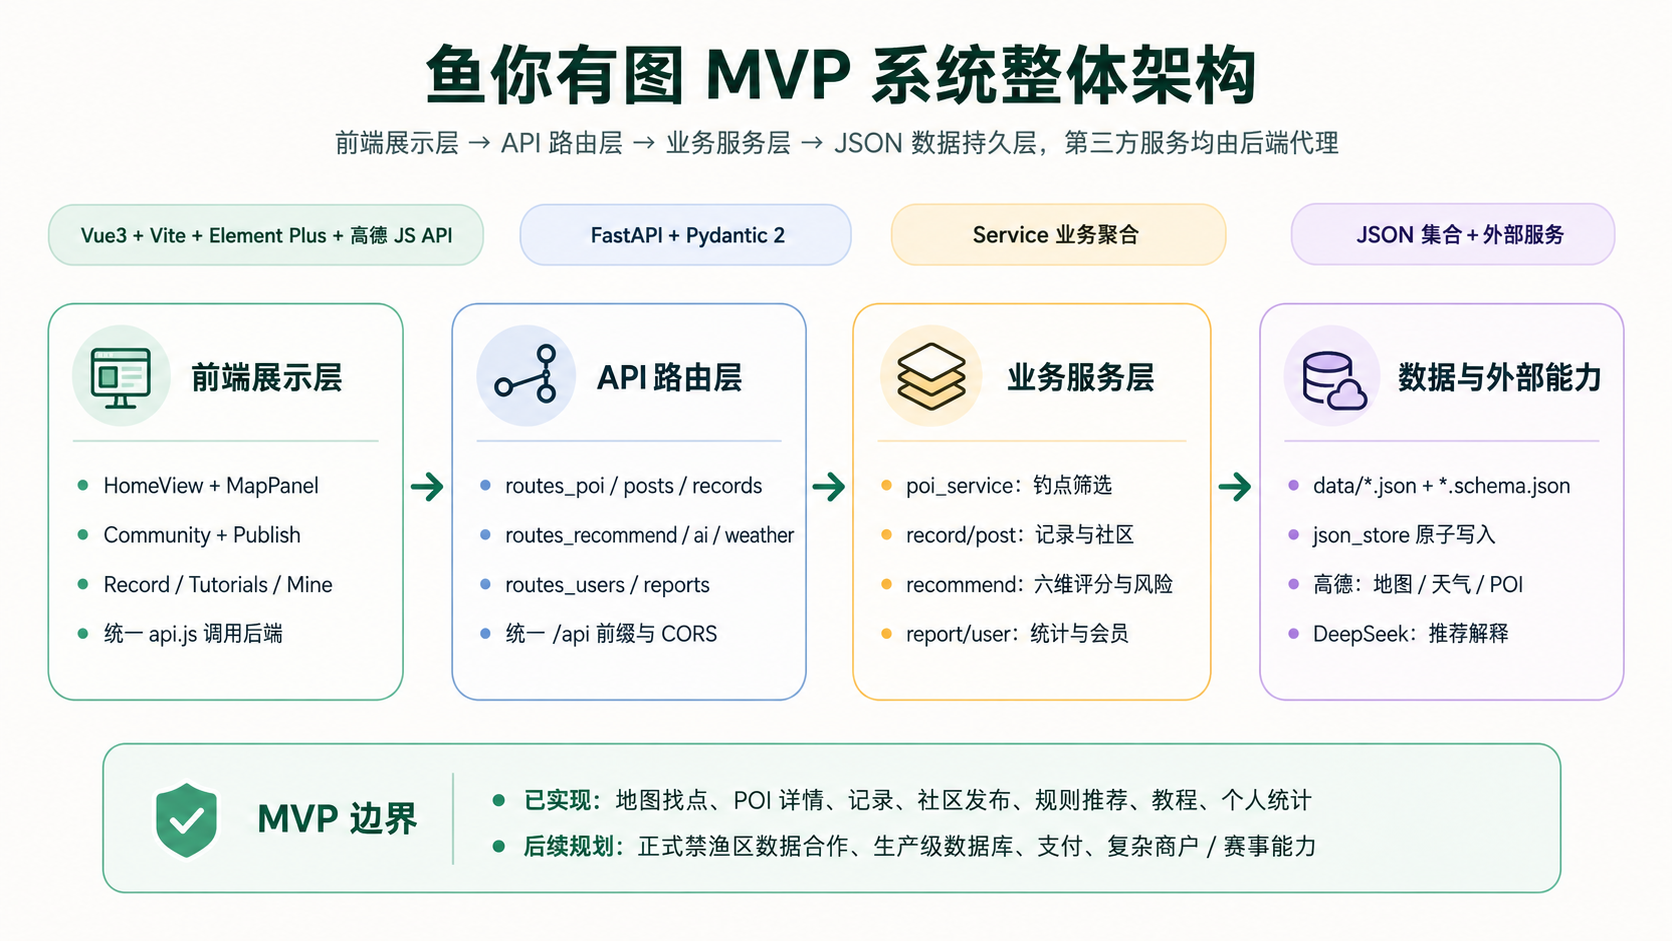
\includegraphics[width=0.9\textwidth]{figures/system_architecture.png}
  \caption{系统整体架构图}
  \label{fig:system-arch}
\end{figure}

\subsection{分层说明}

（待填写：前端展示层、API 网关层、业务服务层、数据持久层的详细说明。）

\subsection{前端架构}

（待填写：Vue 3 + Vite + Element Plus 组件树、状态管理、路由设计。）

\subsection{后端架构}

（待填写：FastAPI 路由注册、Service 层设计、JSON Store 数据层。）

\section{业务与数据流程}

\subsection{核心业务流程}

平台的核心业务闭环为：“打开 App 找钓点 → 判断是否可钓 → 出钓并记录 → 发布分享 → 数据反哺推荐”。

\begin{figure}[H]
  \centering
  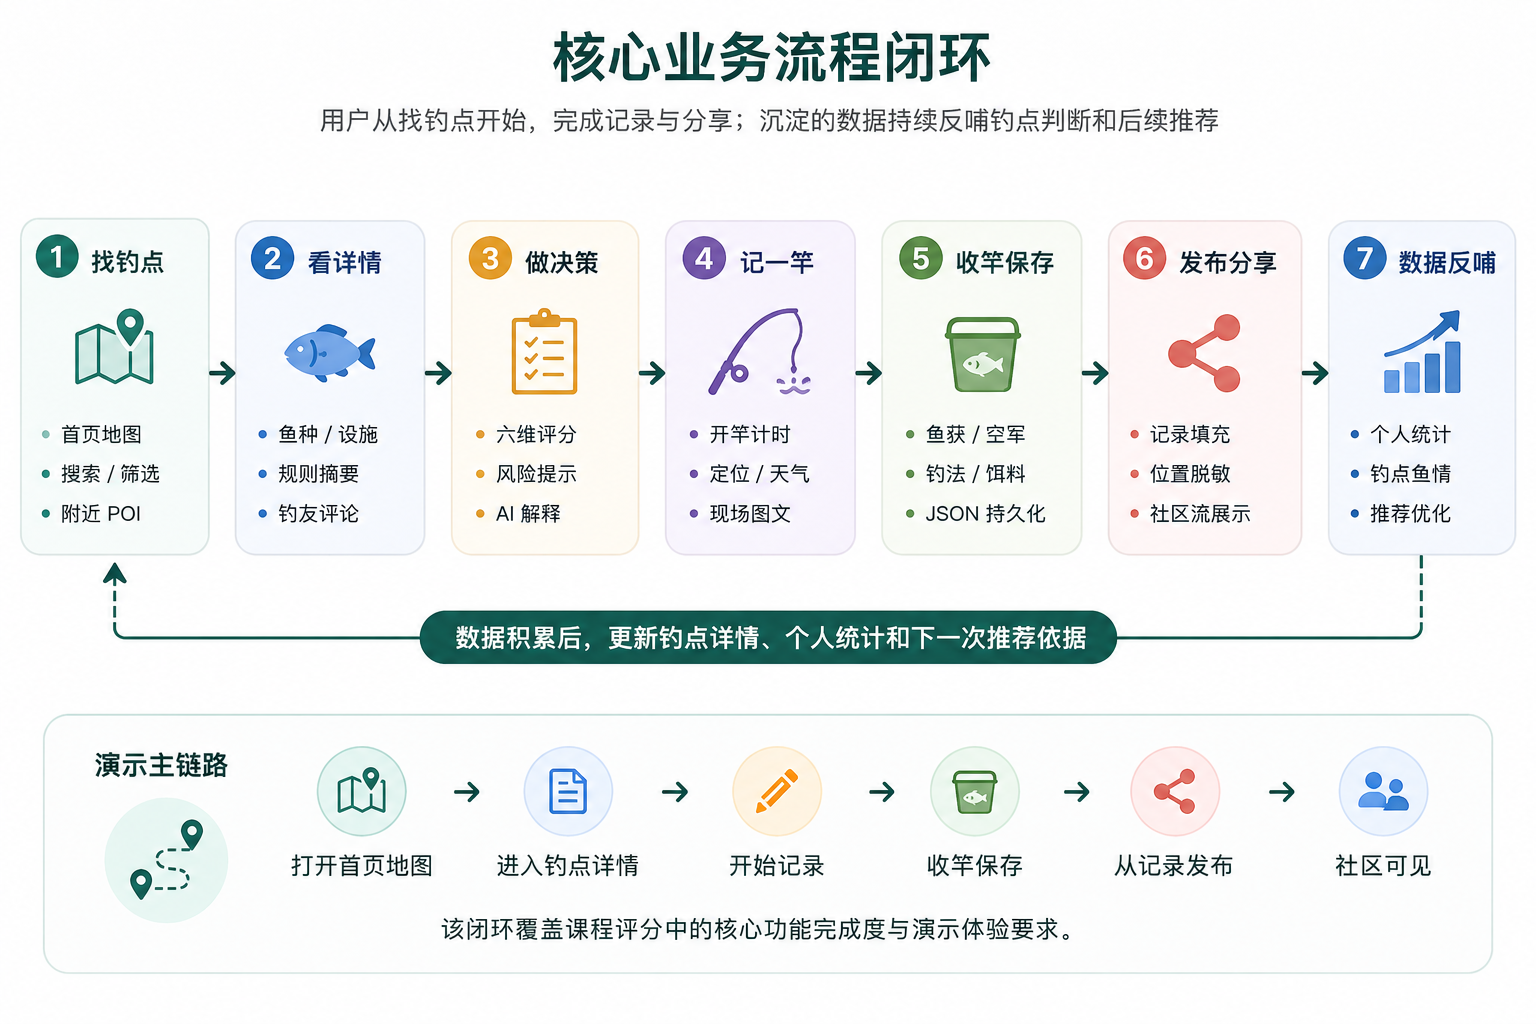
\includegraphics[width=0.85\textwidth]{figures/business_flow.png}
  \caption{核心业务流程图}
  \label{fig:biz-flow}
\end{figure}

\textbf{流程步骤说明：}

\begin{enumerate}
  \item \textbf{找钓点}：用户打开 App，地图首页根据当前位置展示附近钓点。用户可通过搜索、筛选（野钓/钓场/免费/夜钓/路亚等）缩小范围。
  \item \textbf{看详情}：点击 POI 查看钓点详情——名称、类型、距离、鱼种、收费、设施、规则摘要、近期鱼获统计和钓友评价。系统展示推荐理由、合规风险提示和天气适配情况。
  \item \textbf{做决策}：系统根据鱼情分、合规分、距离分、天气适配分、设施便利分和社交热度分计算推荐指数，对 Top 推荐结果由 DeepSeek 生成自然语言建议。禁钓/限钓/极端天气等风险优先提示。
  \item \textbf{出钓记录}：用户到达钓点后，点击“记一竿”开始计时。收竿时填写鱼获信息（鱼种、条数、重量、钓法、饵料）或标记为空军（记录原因和复盘）。天气、时间、位置由系统自动回填。
  \item \textbf{发布分享}：记录完成后可一键生成帖子发布到社区。发布时分别设置内容权限（公开/私密）和位置权限（精确/模糊/隐藏）。生成可分享的战绩卡片。
  \item \textbf{数据沉淀}：鱼获数据进入社区流和钓点详情页，成为其他用户判断该钓点的依据。用户个人主页汇总出钓统计。数据积累后提升推荐准确度。
  \item \textbf{反哺推荐}：形成“用户记录 → 数据沉淀 → 更好推荐 → 更多出钓 → 更多记录”的正向增长闭环。
\end{enumerate}

\subsection{数据流设计}

\begin{figure}[H]
  \centering
  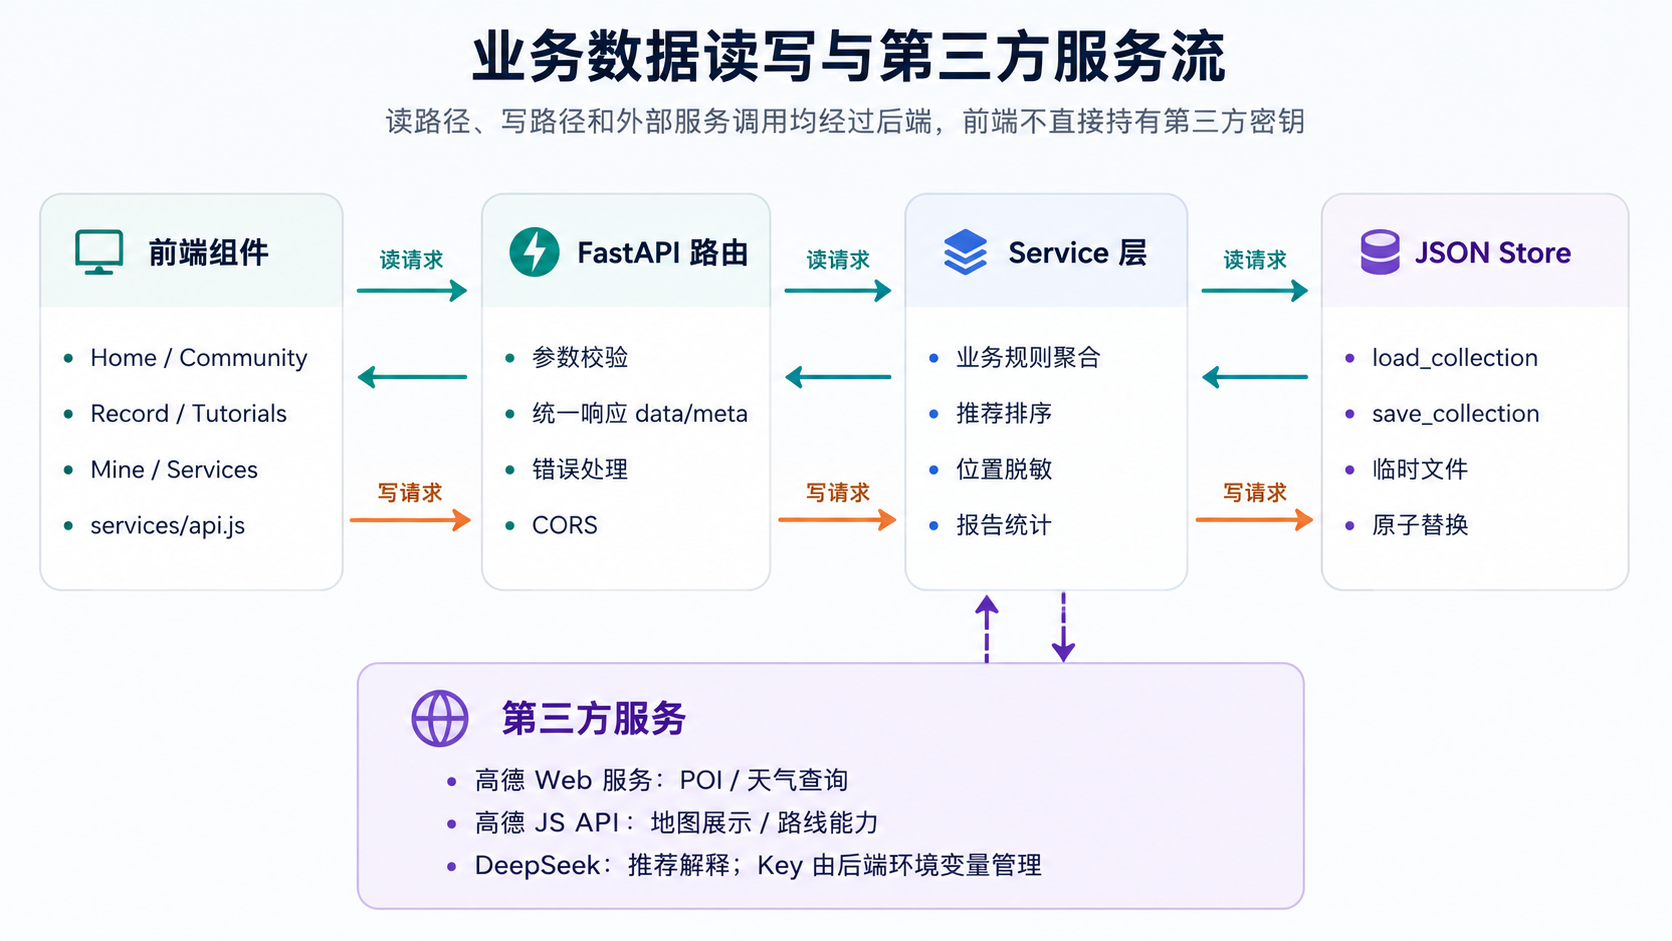
\includegraphics[width=0.85\textwidth]{figures/data_flow.png}
  \caption{数据流架构图}
  \label{fig:data-flow}
\end{figure}

\textbf{数据读写路径：}

\begin{enumerate}
  \item \textbf{读路径}：前端组件 → \texttt{api.js}（HTTP 请求）→ Vite 代理 `/api` → FastAPI 路由 → Service 层调用 \texttt{load\_collection()} → 读取 `data/*.json` → 返回结构化 JSON → 前端渲染
  \item \textbf{写路径}：前端表单提交 → \texttt{api.js} → FastAPI 路由（Pydantic 校验）→ Service 层处理业务逻辑 → \texttt{save\_collection()}（临时文件 + 原子替换）→ 返回写入结果 → 前端更新状态
  \item \textbf{第三方数据接入}：后端 Service 层封装高德 Web 服务（POI 搜索、天气查询）和 DeepSeek API 调用，前端不直接访问第三方服务。当前 MVP 阶段第三方数据以 mock 方式提供，预留真实接口结构。
\end{enumerate}

\subsection{关键数据实体关系}

\begin{table}[H]
  \centering
  \caption{核心数据实体}
  \label{tab:data-entities}
  \begin{tabularx}{\textwidth}{p{3cm}|p{4cm}|p{8cm}}
    \toprule
    \textbf{实体} & \textbf{存储位置} & \textbf{关键关联} \\
    \midrule
    FishingPOI（钓点） & \texttt{data/pois.json} & 被 CatchPost、Recommendation 引用；与高德 POI ID 关联 \\
    \hline
    CatchPost（鱼获记录） & \texttt{data/records.json} & 关联 POI（poi\_id）、用户（user\_id）、天气快照；可作为帖子来源 \\
    \hline
    Post（社区帖子） & \texttt{data/posts.json} & 可关联记录（record\_id）、POI（poi\_id）、用户（user\_id） \\
    \hline
    Recommendation（推荐） & 接口实时生成 & 引用 POI 列表、天气快照、用户偏好摘要 \\
    \hline
    WeatherSnapshot（天气） & \texttt{data/weather\_snapshots.json} & 被 Record、Recommendation 引用 \\
    \hline
    Tutorial（教程） & \texttt{data/tutorials.json} & 关联 POI（练习钓点推荐） \\
    \bottomrule
  \end{tabularx}
\end{table}

实体间核心关系：

\begin{itemize}
  \item 一条 CatchPost 隶属于一个 POI 和一个用户，携带一个天气快照
  \item 一条 Post 可选关联一条 CatchPost（从记录一键生成帖子），此时帖子可追溯到原始出钓数据
  \item 一次 Recommendation 以用户位置和偏好为输入，输出一组候选 POI 及其评分明细
  \item 当前 MVP 阶段以 JSON 文件内 \texttt{\_id} 字段实现实体引用，不引入外键约束
\end{itemize}

\subsection{当前实现状态}

当前 MVP 阶段已实现上述主流程中的关键节点：地图首页展示 POI、POI 详情查看、推荐接口返回评分与理由、记录 CRUD、帖子发布与社区流展示、个人统计汇总。数据持久化通过 JSON 原子写入实现，服务重启后数据不丢失。后续可在现有数据流基础上扩展用户系统、评论/点赞持久化和推荐算法优化。

\section{功能响应表}

本章对照课程实习技术评分表（50 分制，7 个评分维度）逐项说明技术响应情况。每条响应包含：需求项、响应情况（已实现/部分实现/待补充/后续规划）、实现说明和验证方式。

\begin{longtable}{|p{0.5cm}|p{3cm}|p{1.8cm}|p{5cm}|p{3.5cm}|}
  \caption{功能需求响应表}
  \label{tab:func-response}\\
  \toprule
  \textbf{\#} & \textbf{评价项} & \textbf{响应情况} & \textbf{实现说明} & \textbf{验证方式} \\
  \midrule
  \endfirsthead

  \multicolumn{5}{c}{\tablename~\thetable\quad（续）}\\
  \toprule
  \textbf{\#} & \textbf{评价项} & \textbf{响应情况} & \textbf{实现说明} & \textbf{验证方式} \\
  \midrule
  \endhead

  \bottomrule
  \multicolumn{5}{r}{\footnotesize 续下页}\\
  \endfoot

  \bottomrule
  \endlastfoot

  % ===== 维度1：项目定位与需求响应（6分） =====
  1.1 & 围绕五个核心用户问题说明用户场景 & 已实现 & 在产品计划书、功能设计书和本投标文件中明确阐述“去哪钓、能不能钓、现在适不适合钓、钓到了怎么分享和复盘、新手怎么快速上手”五个场景及对应承接模块 & 检查项目概述（第1章）和需求分析（第2章）中的用户场景描述 \\
  \hline
  1.2 & 明确 MVP 边界，不把非 MVP 内容作为当前交付 & 已实现 & 开发设计书和本投标文件明确列出 MVP 范围（地图、POI、记录、社区、推荐、教程）和非 MVP 范围（会员、赛事、商户、遥感、支付等），总体方案章节明确“当前 MVP 阶段已实现”与“后续可扩展”的区别 & 检查开发设计书 MVP 范围声明及本文件第1、3章的边界说明 \\
  \hline

  % ===== 维度2：核心功能完成度（15分） =====
  2.1 & 地图首页与 POI 展示 & 已实现 & 前端 HomeView.vue 与 MapPanel.vue 集成高德 JS API 2.0，展示附近 POI 标记、支持搜索、地图热力表达和天气摘要条；POI 数据通过后端 `/api/pois` 接口从 `data/pois.json` 加载 & 前端运行后进入首页地图，检查 POI 标记、搜索功能和天气摘要 \\
  \hline
  2.2 & 钓点详情 & 已实现 & 点击 POI 展示详情弹窗/页面：名称、类型、距离、鱼种、设施、评分分项、推荐理由、风险提示；数据来自 \texttt{/api/pois/\{poi\_id\}} 接口 & 检查 POI 详情字段完整性，对照 FishingPOI 数据模型 \\
  \hline
  2.3 & 鱼获/空军发布 & 已实现 & RecordView.vue 实现开竿计时和收竿汇总，收竿弹窗支持填写鱼种、条数、重量、钓法、饵料；条数为 0 时标记为空军；后端 `/api/records` POST 接口持久化到 `data/records.json` & 完成一次出钓记录（含鱼获和空军两种情况），重启后端检查数据是否仍存在 \\
  \hline
  2.4 & 社区鱼获流 & 已实现 & CommunityView.vue 展示社区帖子流，支持频道切换（推荐/同城/话题）；PublishView.vue 支持图文发布、关联钓点、内容与位置权限分离；后端 `/api/posts` 和 `/api/feed` 接口 & 发布一条帖子后在社区流中可见，检查帖子与出钓记录的关联 \\
  \hline
  2.5 & 教程页 & 已实现 & TutorialsView.vue 展示教程列表，支持分类筛选（入门/进阶、图文/视频）；数据来自 `data/tutorials.json` & 检查教程列表渲染、分类切换功能 \\
  \hline
  2.6 & 完整流程联动 & 部分实现 & “地图找点 → 详情 → 记录 → 从记录发布 → 社区展示”路径已跑通；记录到帖子的关联（record\_id）已在数据模型中预留并由发布弹层快速填充；个人统计已由前端展示结合后端 profile-summary/report 接口支撑 & 逐步骤演示完整流程，检查各页面间数据传递 \\
  \hline

  % ===== 维度3：技术架构与接口设计（8分） =====
  3.1 & 前后端分离架构 & 已实现 & Vue 3 + Vite 前端与 FastAPI 后端通过 RESTful API 通信；Vite 代理 `/api` 到后端 8000 端口；前端 API 调用集中在 `api.js` & 检查 `vite.config.js` 代理配置和后端路由注册 \\
  \hline
  3.2 & 后端三层架构 & 已实现 & 路由层（`app/api/`）→ 服务层（`app/services/`）→ 数据层（\texttt{app/data/json\_store.py}），职责清晰 & 检查后端目录结构和模块间调用关系 \\
  \hline
  3.3 & API 接口完整性 & 已实现 & 已实现 POI、帖子、记录、推荐、天气、AI 解释、教程等核心接口，统一使用 `data` + `meta` 响应格式 & 通过浏览器开发者工具或接口测试工具检查各端点返回结构 \\
  \hline
  3.4 & 环境变量与密钥管理 & 已实现 & 高德 Key、DeepSeek Key 通过 `.env` 文件由 `config.py` 读取，不写入前端代码；`.env.example` 提供模板 & 检查 `.env` 不在版本控制中，前端无硬编码 Key \\
  \hline

  % ===== 维度4：推荐模型与AI解释设计（7分） =====
  4.1 & 规则模型排序 & 已实现 & 推荐接口 `/api/recommendations` 实现六维评分（鱼情分 0.25、合规分 0.25、距离分 0.15、天气适配分 0.15、设施便利分 0.10、社交热度分 0.10），包含硬性拦截/惩罚项（禁钓、极端天气、岸线安全等） & 检查推荐接口返回的 score、breakdown 和 warnings 字段 \\
  \hline
  4.2 & AI 解释设计 & 部分实现 & AI 接口 `/api/ai/fishing-advice` 已预留结构：接收候选 POI、规则推荐结果和用户意图等结构化数据，返回 JSON 格式的自然语言解释；当前 MVP 阶段若在 production 环境配置 `DEEPSEEK\_API\_KEY` 则可真实调用，否则返回 mock 解释；AI 不参与排序，仅解释推荐结果 & 检查 AI 接口输入参数（不包含用户隐私原文）和输出格式（summary + explanation + top\_recommendations + tips） \\
  \hline
  4.3 & 风险优先提示 & 已实现 & 推荐结果中硬性风险会通过 penalty、warnings 和 POI 内的 risk/risk\_flags 字段体现；存在禁钓/限钓/安全风险的点位会降低排序并提示用户先核对规则与现场安全 & 检查包含禁钓 POI 时的推荐返回结果 \\
  \hline

  % ===== 维度5：数据结构与数据可用性（5分） =====
  5.1 & 核心数据模型 & 已实现 & FishingPOI（20+ 字段，含评分分项和风险标记）、FishingRecord（鱼种/重量/钓法/天气/隐私级别）、CatchPost（帖子内容、关联记录、内容与位置权限）、Recommendation（排名/分项分/理由/警告）、WeatherSnapshot 等模型通过 Pydantic 定义，字段能支撑核心流程 & 检查 `app/schemas/` 目录和接口返回字段 \\
  \hline
  5.2 & JSON 集合与 Schema & 已实现 & 根目录 `data/` 下每个 `.json` 集合配有同名 `.schema.json` 描述文件；当前包含 pois、posts、records、tutorials、weather\_snapshots 等集合 & 检查 `data/` 目录和 schema 文件内容 \\
  \hline
  5.3 & 数据持久化 & 已实现 & \texttt{json\_store.py} 的 \texttt{save\_collection()} 采用临时文件 + 原子替换策略，避免写入中断导致数据损坏；记录和帖子的增删改操作均调用持久化 & 新增记录后重启后端，检查数据仍存在且不重复 \\
  \hline

  % ===== 维度6：界面交互与演示体验（5分） =====
  6.1 & 页面结构与跳转 & 已实现 & 5 个底部 Tab（首页/社区/记录/技巧/服务）覆盖主要页面；“我的”通过顶部菜单抽屉进入，发布通过社区页弹层进入；地图即首页策略，Tab 切换无路由丢失 & 逐 Tab 切换并打开发布弹层、我的抽屉，检查各页面可正常展示 \\
  \hline
  6.2 & 状态反馈 & 部分实现 & 部分组件有加载和空状态处理；错误兜底和离线状态提示尚不完善，当前阶段主要依赖 mock 数据保证演示链路不断裂 & 断网或接口异常时检查页面是否展示错误提示而非白屏 \\
  \hline
  6.3 & 视觉统一性 & 已实现 & 统一使用 Element Plus 组件库，配色和布局保持一致性 & 检查各页面截图，对照视觉风格 \\
  \hline

  % ===== 维度7：文档规范与团队协作（4分） =====
  7.1 & 文档完整性 & 已实现 & 已输出产品计划书、功能设计书、开发设计书、技术评分表、技术投标文件（本文件），覆盖课程要求文档清单 & 对照课程文档要求逐项核对 \\
  \hline
  7.2 & 内容与实现一致 & 已实现 & 文档描述的功能模块、数据模型、API 接口、页面结构与实际代码一致；非 MVP 内容明确标注为“后续规划” & 随机抽取文档中的功能描述，在代码中验证是否存在对应实现 \\
  \hline
  7.3 & 编号与格式统一 & 已实现 & 本文件采用连续章节编号，表格使用统一样式（tabularx/longtable），功能响应表包含“需求项、响应情况、实现说明、验证方式”四列 & 检查文件目录、交叉引用和表格格式 \\
  \bottomrule
\end{longtable}

\section{核心功能详细设计}

\subsection{地图与 POI 模块}

（待填写：高德地图集成方案、POI 搜索与展示、禁渔区查询、钓点详情页设计。）

\subsection{出钓记录模块}

（待填写：开竿计时、收竿汇总、鱼获录入、空军标记、场景模板（湖钓/海钓）、图片上传。）

\subsection{社区与发布模块}

（待填写：帖子发布、内容权限与位置隐私设置、评论/点赞/关注、信息流。）

\subsection{推荐与 AI 模块}

（待填写：规则模型排序、DeepSeek API 接入、鱼情预测、个性化推荐。）

\subsection{个人主页与会员报告}

（待填写：单级会员体系、偏好与效率分析、月报/年报/生涯报告、分享卡导出。）

\subsection{教程与装备模块}

（待填写：教程列表与学习进度、装备履历、商家服务。）

\subsection{活动与社群模块}

（待填写：活动创建与报名、签到、活动群聊。）

\section{数据模型与接口设计}

本章说明平台在 PostgreSQL + PostGIS 数据库下的数据模型、字段结构和接口规范。数据设计围绕“地图找点、规则判断、个性化推荐、出钓记录、社区分享、教程学习、活动服务”七类业务展开，要求结构清晰、字段可验证、空间查询可计算、隐私权限可控制。

\subsection{数据库设计原则}

数据库采用 PostgreSQL 作为主数据库，启用 PostGIS 扩展处理地理空间数据。PostgreSQL 负责保存用户、钓点、鱼种、出钓记录、帖子、教程、活动、订单、报告等结构化数据；PostGIS 负责钓点坐标、水域边界、禁钓区域、附近检索和空间叠加判断。

数据库设计遵循以下原则：

\begin{enumerate}
  \item \textbf{主数据稳定：}用户、钓点、鱼种、教程、装备等相对稳定数据采用独立主表维护，避免在记录和帖子中重复保存大量冗余信息。
  \item \textbf{业务数据可追溯：}出钓记录、社区帖子、评论、点赞、报告快照等业务数据保留创建时间、更新时间、操作者和状态字段，支撑统计分析与审计追踪。
  \item \textbf{空间数据可计算：}钓点、水域和禁钓区使用 PostGIS 几何字段保存，支持附近点位查询、距离排序、点面叠加和空间范围过滤。
  \item \textbf{隐私字段分级：}用户精确位置、私密记录、私信内容、图片地址等敏感字段与公开展示字段分开处理，接口返回时按权限和位置可见性进行脱敏。
  \item \textbf{扩展字段可控：}对于推荐结果、报告快照、第三方返回摘要等半结构化内容，采用 \texttt{jsonb} 保存，但核心关联关系仍通过关系表和外键表达。
\end{enumerate}

\subsection{核心数据表设计}

数据库表按业务域划分为用户与关系、垂钓主数据、记录与社区、推荐与报告、活动与服务、系统配置六类。

{\small
\begin{longtable}{|>{\raggedright\arraybackslash}p{3.9cm}|>{\raggedright\arraybackslash}p{3.0cm}|>{\raggedright\arraybackslash}p{6.7cm}|}
  \caption{数据库核心表设计}
  \label{tab:postgres-tables}\\
  \toprule
  \textbf{表名} & \textbf{用途} & \textbf{主要字段设计} \\
  \midrule
  \endfirsthead
  \multicolumn{3}{c}{\tablename~\thetable\quad（续）}\\
  \toprule
  \textbf{表名} & \textbf{用途} & \textbf{主要字段设计} \\
  \midrule
  \endhead
  \bottomrule
  \endlastfoot
  users & 用户基础信息 & id、nickname、avatar、phone\_hash、city、level、status、created\_at、updated\_at \\
  \hline
  user\_preferences & 用户个性化偏好 & user\_id、target\_fish、preferred\_methods、distance\_limit\_m、privacy\_default、risk\_tolerance、updated\_at \\
  \hline
  memberships & 会员状态与权益 & user\_id、member\_level、valid\_until、benefits、status、created\_at \\
  \hline
  fishing\_pois & 垂钓 POI 主表 & id、name、type、city、district、address、lng、lat、geom、fish、tags、score、facilities、is\_banned、compliance\_note、updated\_at \\
  \hline
  fishing\_areas & 水域与禁钓区域 & id、name、area\_type、city、geom、rule\_text、rule\_source、effective\_from、effective\_to、status \\
  \hline
  fish\_species & 鱼种知识库 & id、name、alias、habitat、active\_temperature、common\_methods、bait\_tips、season\_tips \\
  \hline
  weather\_snapshots & 天气快照 & id、city、adcode、weather、temperature\_c、wind\_level、humidity、pressure\_hpa、alerts、source、updated\_at \\
  \hline
  fishing\_records & 出钓记录 & id、user\_id、poi\_id、start\_time、end\_time、duration\_seconds、fish\_count、fish\_weight、method、bait、is\_blank\_trip、privacy\_level、location\_geom \\
  \hline
  catch\_entries & 单尾鱼获明细 & id、record\_id、species、weight、length\_cm、caught\_at、image\_url、note \\
  \hline
  posts & 社区帖子 & id、user\_id、post\_type、title、content、poi\_id、record\_id、visibility、location\_visibility、location\_text、display\_geom、created\_at \\
  \hline
  comments & 评论数据 & id、post\_id、user\_id、content、parent\_id、status、created\_at \\
  \hline
  reactions & 点赞、收藏等互动 & id、target\_type、target\_id、user\_id、reaction\_type、created\_at \\
  \hline
  recommendation\_logs & 推荐结果日志 & id、user\_id、request\_json、result\_json、agent\_version、created\_at \\
  \hline
  report\_snapshots & 个人报告快照 & id、user\_id、period、summary\_json、generated\_at、source \\
  \hline
  tutorials & 教程内容 & id、title、category、difficulty、format、duration、content、related\_poi\_ids、status \\
  \hline
  learning\_progress & 学习进度 & id、user\_id、tutorial\_id、status、practice\_notes、updated\_at \\
  \hline
  events & 活动信息 & id、title、city、poi\_id、start\_time、capacity、fee、safety\_notice、status \\
  \hline
  event\_registrations & 活动报名 & id、event\_id、user\_id、status、checked\_in\_at、created\_at \\
  \hline
  groups、messages & 活动群与消息 & group\_id、user\_id、content、message\_type、read\_status、created\_at \\
  \hline
  equipment、orders & 装备与订单 & equipment\_id、user\_id、quantity、order\_status、pay\_status、created\_at \\
\end{longtable}
}

\subsection{字段约束与索引设计}

空间字段使用 WGS84 坐标系，钓点位置采用 \texttt{geometry(Point, 4326)}，水域和禁钓区域采用 \texttt{geometry(Polygon, 4326)} 或 \texttt{geometry(MultiPolygon, 4326)}。\texttt{fishing\_pois.geom}、\texttt{fishing\_areas.geom} 建立 GiST 索引，用于附近检索和点面叠加判断。用户、记录、帖子、活动等高频查询字段建立 B-tree 索引，例如 \texttt{user\_id}、\texttt{poi\_id}、\texttt{created\_at}、\texttt{status}、\texttt{post\_type}。

关键约束包括：用户 ID、POI ID、记录 ID 和帖子 ID 采用全局唯一标识；记录开始时间不得晚于结束时间；鱼获数量和重量不得为负；帖子位置展示字段必须与 \texttt{location\_visibility} 保持一致；订单、活动报名、学习进度等状态字段使用枚举约束，防止非法状态进入业务流程。

\subsection{核心数据模型}

出钓记录是连接地图、推荐、报告和社区的核心数据。记录中既保存用户填写的鱼种、重量、钓法、饵料，也保存与 POI、天气和位置相关的结构化字段，用于个性化推荐和生涯统计。

\begin{lstlisting}[caption={出钓记录数据模型示例},label={lst:record-schema}]
{
  "id": "rec_001",
  "user_id": "u_001",
  "start_time": "2026-07-01T06:30:00",
  "end_time": "2026-07-01T10:45:00",
  "duration_seconds": 15300,
  "poi_id": "poi_wh_001",
  "location_name": "东湖磨山水域",
  "latitude": 30.5501,
  "longitude": 114.4085,
  "weather": "多云",
  "temperature": 28,
  "fish_count": 12,
  "fish_weight": 3.8,
  "fish_species": "鲫鱼,鲤鱼",
  "fishing_method": "台钓",
  "bait": "商品饵",
  "is_blank_trip": false,
  "privacy_level": "private"
}
\end{lstlisting}

\subsection{API 接口总览}

后端采用 FastAPI 提供统一 \texttt{/api} 前缀，接口以 RESTful 风格组织。接口覆盖地图 POI、天气、推荐、AI 解释、出钓记录、社区帖子、教程、用户报告、活动和服务订单等模块。

\begin{longtable}{|p{0.7cm}|p{3.5cm}|p{2.5cm}|p{3.9cm}|p{2.0cm}|}
  \caption{API 接口总览表}
  \label{tab:api-list}\\
  \toprule
  \textbf{序号} & \textbf{接口路径} & \textbf{方法} & \textbf{功能} & \textbf{所属模块} \\
  \midrule
  \endfirsthead
  \multicolumn{5}{c}{\tablename~\thetable\quad（续）}\\
  \toprule
  \textbf{序号} & \textbf{接口路径} & \textbf{方法} & \textbf{功能} & \textbf{所属模块} \\
  \midrule
  \endhead
  \bottomrule
  \endlastfoot
  1 & \path|/api/health| & {\scriptsize GET} & 服务健康检查 & 元数据 \\
  \hline
  2 & \path|/api/amap/config| & {\scriptsize GET} & 返回前端加载高德 JS API 所需配置 & 地图配置 \\
  \hline
  3 & \path|/api/pois| & {\scriptsize GET} & 查询钓点列表，支持城市、关键词、距离等条件 & 地图 POI \\
  \hline
  4 & \path|/api/pois/{poi_id}| & {\scriptsize GET} & 查询钓点详情 & 地图 POI \\
  \hline
  5 & \path|/api/weather/current| & {\scriptsize GET} & 获取实时天气快照 & 天气服务 \\
  \hline
  6 & \path|/api/recommendations| & {\scriptsize POST} & 根据位置、偏好、天气和候选 POI 返回推荐排序 & 推荐模型 \\
  \hline
  7 & \path|/api/ai/fishing-advice| & {\scriptsize POST} & 根据推荐结果生成个性化出钓建议 & AI Agent \\
  \hline
  8 & \path|/api/records| & {\scriptsize GET/POST} & 查询和新增出钓记录 & 出钓记录 \\
  \hline
  9 & \path|/api/records/{record_id}| & {\scriptsize\begin{tabular}[t]{@{}l@{}}GET\\PATCH\\DELETE\end{tabular}} & 查询、更新和删除单条出钓记录 & 出钓记录 \\
  \hline
  10 & \path|/api/posts| & {\scriptsize GET/POST} & 查询和发布社区帖子 & 社区 \\
  \hline
  11 & \path|/api/feed| & {\scriptsize GET} & 获取社区信息流 & 社区 \\
  \hline
  12 & \path|/api/posts/{post_id}| & {\scriptsize GET} & 查询帖子详情 & 社区 \\
  \hline
  13 & \path|/api/posts/{post_id}/comments| & {\scriptsize GET/POST} & 查询或新增评论 & 社区互动 \\
  \hline
  14 & \path|/api/posts/{post_id}/reactions| & {\scriptsize POST} & 点赞、收藏等互动 & 社区互动 \\
  \hline
  15 & \path|/api/tutorials| & {\scriptsize GET} & 查询教程列表 & 教程 \\
  \hline
  16 & \path|/api/tutorials/{tutorial_id}/progress| & {\scriptsize PUT} & 更新学习进度 & 教程 \\
  \hline
  17 & \path|/api/users/{user_id}| & {\scriptsize GET} & 查询用户基础信息 & 用户 \\
  \hline
  18 & \path|/api/users/{user_id}/profile-summary| & {\scriptsize GET} & 获取个人统计摘要 & 个人报告 \\
  \hline
  19 & \path|/api/users/{user_id}/reports| & {\scriptsize GET/POST} & 查询或生成报告快照 & 个人报告 \\
  \hline
  20 & \path|/api/fish-species| & {\scriptsize GET} & 查询鱼种知识库 & 知识库 \\
\end{longtable}

\subsection{接口规范}

接口响应统一采用“业务数据 + 元信息”的结构。列表接口返回 \texttt{data} 数组和 \texttt{meta} 元信息；详情接口返回单个 \texttt{data} 对象；创建接口成功时返回新建对象并使用 HTTP 201 状态码；删除接口成功时返回 HTTP 204。错误响应统一包含错误码、错误信息和请求追踪 ID，便于前端展示和后端排查。

\begin{lstlisting}[caption={列表接口返回结构示例},label={lst:list-response}]
{
  "data": [
    {
      "id": "poi_wh_001",
      "name": "东湖磨山水域",
      "score": 86
    }
  ],
  "meta": {
    "total": 1,
    "page": 1,
    "page_size": 20
  }
}
\end{lstlisting}

分页参数统一采用 \texttt{page}、\texttt{page\_size}；筛选参数按模块扩展，例如 POI 接口支持 \texttt{city}、\texttt{keyword}、\texttt{lat}、\texttt{lng}、\texttt{radius\_m}，帖子接口支持 \texttt{channel}、\texttt{post\_type}，记录接口支持 \texttt{user\_id}。接口错误处理遵循 HTTP 状态码语义：400 表示请求参数错误，401 表示未认证，403 表示无权限，404 表示资源不存在，409 表示状态冲突，500 表示服务端异常。生产环境中错误响应不返回堆栈和敏感配置。



\section{推荐算法与 AI 能力}

\subsection{推荐系统设计}

（待填写：规则模型排序策略、多因子评分（距离、天气、禁渔规则、历史鱼获、社区活跃度）、推荐接口设计。）

\subsection{AI 钓鱼建议}

（待填写：DeepSeek API 接入方案、提示词设计、AI 建议输出格式、Mock 降级策略。）

\subsection{偏好与效率分析}

（待填写：偏好指标（最常用钓法、最常出钓时段）与效率指标（单位小时鱼获、空军率）的算法区分。）

\begin{table}[H]
  \centering
  \caption{偏好分析 vs 效率分析}
  \label{tab:analysis-compare}
  \begin{tabularx}{0.85\textwidth}{p{2.5cm}|X|X}
    \toprule
    \textbf{维度} & \textbf{偏好分析} & \textbf{效率分析} \\
    \midrule
    计算方法 & 按记录出现次数统计 & 按单位时间产出计算 \\
    \midrule
    典型指标 & 最常用钓法、常钓鱼种、偏好时段 & 最高效钓法、最佳时段、最低空军率条件 \\
    \midrule
    数据要求 & 至少 1 条记录 & 至少 5 条有效记录 \\
    \bottomrule
  \end{tabularx}
\end{table}

\section{技术选型}

本章说明“鱼你有图”项目的技术栈、选型理由和工程适配关系。选型原则是采用成熟、稳定、便于部署和便于团队维护的技术组合，使地图服务、空间数据、推荐模型、AI Agent、社区内容和用户数据能够形成统一的工程闭环。

\subsection{技术栈总览}

\begin{table}[H]
  \centering
  \caption{技术栈总览}
  \label{tab:tech-stack}
  \begin{tabularx}{\textwidth}{p{3cm}|p{4.6cm}|X}
    \toprule
    \textbf{层次} & \textbf{技术选型} & \textbf{说明} \\
    \midrule
    前端框架 & Vue 3 + Vite & 构建移动端优先的单页应用，支撑地图、社区、记录、教程和个人中心等页面 \\
    \hline
    UI 组件库 & Element Plus + 图标组件 & 提供表单、弹窗、标签、按钮、图标等基础控件，保证页面风格统一 \\
    \hline
    地图能力 & 高德 JS API 2.0 + 高德 Web Service & 前端负责地图渲染，后端封装 POI、天气、地理编码等服务调用 \\
    \hline
    后端框架 & Python 3.11 + FastAPI + Pydantic 2 & 提供类型清晰的 RESTful API，适合规则推荐、AI Agent 和第三方服务封装 \\
    \hline
    数据库 & PostgreSQL + PostGIS & 保存业务数据和空间数据，支撑附近查询、空间索引、禁钓区域判断和推荐排序 \\
    \hline
    数据访问与迁移 & SQLAlchemy 2 + Alembic & 统一数据库模型、查询逻辑和表结构版本管理 \\
    \hline
    缓存与会话 & Redis & 缓存天气、热点 POI、推荐结果、登录会话和限流计数 \\
    \hline
    对象存储 & OSS/S3 兼容对象存储 & 存放鱼获图片、帖子图片、头像、教程视频封面和报告长图 \\
    \hline
    AI 服务 & DeepSeek API & 生成个性化出钓建议、推荐解释和复盘摘要，不直接决定排序 \\
    \hline
    网关与部署 & Nginx + HTTPS & 托管前端静态资源，反向代理 \texttt{/api}，处理 HTTPS 和访问日志 \\
    \hline
    测试与质量 & Pytest + 前端构建检查 & 覆盖后端服务、数据模型、推荐规则、权限控制和前端构建质量 \\
    \bottomrule
  \end{tabularx}
\end{table}

\subsection{前端选型理由}

前端采用 Vue 3 + Vite。Vue 组件模型清晰、学习成本适中、生态成熟，适合构建地图首页、钓点详情、社区信息流、发布表单、出钓记录、教程列表和个人报告等页面。Vite 提供快速构建和模块化开发能力，便于团队在页面交互、地图组件和 API 调用之间保持清晰边界。

Element Plus 用于基础控件和交互组件，能够减少重复开发，使页面风格、表单校验、弹窗交互和状态提示保持一致。地图类页面由高德 JS API 承接，普通业务页面由 Vue 组件承接，二者通过统一状态和 API 服务层协作。

\subsection{后端选型理由}

后端采用 FastAPI。FastAPI 与 Pydantic 结合后，可以直接定义 POI、记录、帖子、推荐、天气、用户偏好等模型，接口参数和响应结构清晰，适合投标文件、接口文档和代码实现保持一致。Python 生态对规则模型、统计分析、AI API 调用和数据处理友好，能够支撑推荐 Agent 的快速迭代。

后端分为 API 路由层、业务服务层、数据访问层和第三方服务封装层。API 路由层处理 HTTP 请求和参数校验；业务服务层承接推荐、记录、社区、报告和权限逻辑；数据访问层通过 SQLAlchemy 操作 PostgreSQL；第三方封装层统一接入高德、DeepSeek、对象存储和通知服务。

\subsection{数据库选型理由}

数据持久化采用 PostgreSQL + PostGIS。PostgreSQL 具备成熟的事务、索引、约束和备份能力，适合保存用户、记录、帖子、评论、活动、订单等关系明确的数据。PostGIS 提供空间类型、空间索引和空间函数，能够直接支撑附近钓点查询、禁钓区叠加判断、水域范围筛选和位置脱敏等 GIS 场景。

相比 MySQL，PostgreSQL + PostGIS 在空间数据处理方面更适合本项目；相比 MongoDB，关系型数据库更便于维护用户、记录、帖子、活动报名、互动数据之间的关联一致性。对于推荐结果、报告快照和第三方摘要等半结构化内容，PostgreSQL 的 \texttt{jsonb} 字段能够兼顾灵活性和查询能力。

\subsection{AI 与推荐选型理由}

推荐系统采用规则模型与 AI Agent 分工协作。规则模型负责可解释排序、合规拦截和风险降权，避免推荐结果不可验证；AI Agent 负责解释推荐原因、结合用户偏好生成出钓建议、形成复盘摘要和教程建议。该设计既能体现智能化服务能力，也能保证合规、安全和可审计。

DeepSeek API 用于自然语言生成。后端只向大模型传递结构化上下文和授权画像摘要，不传递完整隐私原文。大模型输出必须经过格式校验和风险约束，不允许直接覆盖规则排序结果。

\subsection{部署与运维选型理由}

Nginx 负责前端静态资源托管、HTTPS 终止、反向代理和访问日志。Redis 用于缓存热点数据、天气快照、推荐结果和限流计数，降低数据库和第三方服务压力。对象存储用于保存图片、视频、头像和报告长图，数据库仅保存文件元数据和访问地址。

Alembic 负责数据库迁移脚本管理，保证不同环境表结构一致；Pytest 用于后端单元测试和接口测试；前端构建检查用于保证页面资源可正常打包。通过这些技术组合，系统能够支撑课程交付、线上运行和生产部署。


\section{第三方服务集成}

本章说明平台第三方服务的接入方式、责任边界、密钥管理和降级策略。第三方能力主要用于地图底图、POI 检索、天气快照、对象存储、HTTPS 证书和 AI 解释生成。系统设计要求第三方服务由后端统一封装，前端只获取必要的展示配置和业务结果，避免 Web 服务 Key、AI Key 等敏感信息暴露在前端代码中。

\subsection{高德地图服务}

高德地图服务分为前端 JS API 和后端 Web Service 两类能力。

\textbf{高德 JS API 2.0：}用于前端地图渲染、标记点展示、地图拖动缩放、关键字搜索体验和地图交互。首页地图、POI 标记、钓点详情入口和位置选择均基于该能力实现。前端加载地图所需配置通过 \texttt{/api/amap/config} 获取，不在页面中硬编码真实 Key。

\textbf{高德 Web Service：}由后端封装，用于 POI 搜索、周边检索、天气查询、地理编码和逆地理编码。Web Service Key 只保存在服务端环境变量中，前端不得直接调用带密钥的 Web 服务接口。

\begin{table}[H]
  \centering
  \caption{高德服务接入责任划分}
  \label{tab:amap-integration}
  \begin{tabularx}{\textwidth}{p{3cm}|p{4cm}|X}
    \toprule
    \textbf{能力} & \textbf{接入位置} & \textbf{设计说明} \\
    \midrule
    地图底图与标记渲染 & 前端 & 使用高德 JS API 2.0 渲染地图、POI 标记和交互状态 \\
    \hline
    JS API 配置下发 & 后端 & \texttt{/api/amap/config} 返回前端必要配置，便于环境隔离和集中管理 \\
    \hline
    POI 周边检索 & 后端 & 后端调用高德 Web Service，并结合自建垂钓 POI 做语义增强 \\
    \hline
    天气查询 & 后端 & 天气结果转换为统一 \texttt{WeatherSnapshot}，供推荐模型和页面摘要使用 \\
    \hline
    地理编码与逆地理编码 & 后端 & 用于记录位置回填、城市识别、地址展示和位置隐私模糊表达 \\
    \bottomrule
  \end{tabularx}
\end{table}

高德 POI 提供通用地图点位，平台在此基础上叠加鱼种、设施、规则、风险、用户记录和社区热度，形成垂钓语义 POI。高德结果不直接等同于官方可钓点，合规判断必须结合平台维护的规则字段和公开管理要求。

\subsection{DeepSeek API}

DeepSeek API 用于生成推荐解释、个性化出钓建议和复盘摘要。系统不把大模型作为排序器，也不让大模型生成未经校验的禁钓结论。DeepSeek 请求由后端统一封装，核心控制项如下：

\begin{itemize}
  \item \textbf{密钥管理：}通过 \texttt{DEEPSEEK\_API\_KEY} 环境变量配置，不写入代码、不传给前端。
  \item \textbf{模型选择：}通过 \texttt{DEEPSEEK\_MODEL} 控制，默认使用稳定的对话模型，便于统一替换和灰度发布。
  \item \textbf{超时控制：}后端调用设置超时时间，避免 AI 服务慢响应影响主流程。
  \item \textbf{输入控制：}只传规则推荐结果、候选 POI 摘要、天气摘要、用户意图和授权画像摘要，不传完整隐私数据。
  \item \textbf{输出控制：}要求返回结构化 JSON，前端只渲染指定字段，并由后端进行格式校验。
\end{itemize}

\subsection{天气与环境数据服务}

天气数据通过后端统一接口获取和标准化，不让业务层直接依赖第三方返回结构。天气字段包括城市、天气现象、温度、体感温度、风向、风力、湿度、气压、能见度、预警信息和更新时间。

推荐模型使用天气数据时只做适宜度判断，不输出“必定爆护”等不可验证表述。遇到雷雨、大风、台风、暴雨等风险天气时，系统优先提示安全风险，并在推荐排序中降低户外野钓点位优先级。

\subsection{对象存储与 CDN}

鱼获图片、帖子图片、用户头像、教程视频封面和报告长图存放在对象存储中，并通过 CDN 加速访问。数据库只保存文件 URL、文件类型、大小、归属用户、关联业务 ID 和审核状态，不直接存放大文件。

对象存储集成策略如下：

\begin{itemize}
  \item 上传由后端生成受控上传地址或统一代理上传，限制文件类型、大小和数量。
  \item 私密记录图片不直接公开访问，需结合权限校验或短期签名 URL。
  \item 删除帖子或记录时，业务数据先软删除，文件清理由异步任务处理，避免误删。
  \item 图片访问地址与审核状态绑定，未通过审核的图片不进入公开社区流。
\end{itemize}

\subsection{HTTPS、域名与证书}

平台通过 HTTPS 提供服务，避免用户位置、登录凭证、发帖内容和图片上传信息在传输过程中被窃听或篡改。Nginx 负责 HTTPS 终止、证书自动续期、静态资源托管、访问日志和 \texttt{/api} 反向代理。

\subsection{服务降级策略}

第三方服务不可用时，系统应保持核心流程可访问。降级策略如下：

\begin{longtable}{|p{3cm}|p{4.5cm}|p{6cm}|}
  \caption{第三方服务降级策略}
  \label{tab:third-party-fallback}\\
  \toprule
  \textbf{服务} & \textbf{异常场景} & \textbf{降级方案} \\
  \midrule
  \endfirsthead
  \multicolumn{3}{c}{\tablename~\thetable\quad（续）}\\
  \toprule
  \textbf{服务} & \textbf{异常场景} & \textbf{降级方案} \\
  \midrule
  \endhead
  \bottomrule
  \endlastfoot
  高德 JS API & 地图加载失败、Key 配置错误 & 前端展示钓点列表和错误提示，不影响查看 POI 文本信息 \\
  \hline
  高德 POI 服务 & 周边搜索失败或超时 & 使用平台自建 POI 和缓存数据，提示用户稍后刷新地图结果 \\
  \hline
  天气服务 & 天气接口失败 & 使用最近一次天气快照或展示天气未知，推荐模型降低天气因子权重 \\
  \hline
  DeepSeek API & 超时、限额、异常 & 返回规则模型解释模板，推荐排序结果不受影响 \\
  \hline
  对象存储/CDN & 图片上传或访问失败 & 保留文本记录和帖子，图片显示占位图，后台重试上传 \\
\end{longtable}

通过以上设计，第三方服务增强用户体验，但不成为核心业务闭环的单点故障。

\section{安全、隐私与合规}

\subsection{数据安全}

（待填写：API Key 管理、密钥不硬编码、HTTPS 传输、数据备份策略。）

\subsection{位置隐私保护}

（待填写：四级位置精度控制（精确/水域模糊/仅城市/完全隐藏）、后端脱敏逻辑、前端与后端双重保障。）

\subsection{用户鉴权}

（待填写：基础鉴权方案、防止越权操作的校验机制。）

\subsection{合规性}

（待填写：《个人信息保护法》合规、禁渔区数据合规、用户内容审核机制。）

\section{部署与运行方案}

本项目部署与运行方案以“课程验收可复现、核心链路可演示、配置边界清晰、第三方异常可降级”为原则。本期交付采用 Vue 3 + Vite 前端、FastAPI 后端、根目录 \texttt{data/} JSON 集合和高德/DeepSeek 可选第三方服务，不使用 Docker，也不在本期强制引入 PostgreSQL、Redis、对象存储或正式网关。

\subsection{运行环境}

课程验收环境划分为本地开发环境和演示测试环境两类。

\begin{itemize}
  \item \textbf{本地开发环境：}前端通过 \texttt{npm install} 和 \texttt{npm run dev} 启动，Vite 默认端口为 5173；后端在 conda 环境 \texttt{fish} 中进入 \texttt{backend} 目录，通过 \texttt{uvicorn app.main:app --reload --host 127.0.0.1 --port 8000} 启动。
  \item \textbf{演示测试环境：}可在同一主机或测试服务器上运行前端构建产物与 FastAPI 服务，使用统一的环境变量文件配置高德和 DeepSeek Key。若未配置真实 Key，系统应使用内置演示数据或 mock 解释保持主流程可演示。
\end{itemize}

当前 MVP 阶段根目录 \texttt{data/} 使用 JSON 模拟 NoSQL 数据库，每个 \texttt{.json} 对应一个集合，每个 \texttt{.schema.json} 对应集合字段说明。JSON 文件适合课堂 Demo 和单机演示，不承诺正式多人并发写入能力。

\subsection{本期部署拓扑}

本期部署拓扑为：浏览器访问 Vue 3 + Vite 前端页面；前端通过 \texttt{api.js} 访问 \texttt{/api}；Vite 开发代理或测试环境反向代理将请求转发到 FastAPI；FastAPI 路由调用 Service 层；Service 层读取或写入 JSON 集合，并按需调用高德或 DeepSeek 服务。推荐排序由后端规则模型完成，AI 只负责解释生成，不直接改变排序。

第三方 Key 均通过后端环境变量配置，不允许出现在 Git 仓库、前端打包文件、公开截图和测试报告中。高德 JS API 配置由 \texttt{/api/amap/config} 下发；高德 Web Service Key 和 DeepSeek Key 只保存在后端环境变量中。

\subsection{配置项与启动检查}

后端至少需要检查以下配置项，配置项清单见表 \ref{tab:config-items}。

\begin{table}[htbp]
  \centering\small
  \caption{核心配置项清单}
  \label{tab:config-items}
  \begin{tabularx}{\textwidth}{>{\raggedright\arraybackslash}p{2.8cm}|>{\raggedright\arraybackslash}p{1.5cm}|X|>{\raggedright\arraybackslash}p{2.8cm}|>{\raggedright\arraybackslash}p{1.2cm}}
    \toprule
    \textbf{配置项} & \textbf{类型} & \textbf{说明} & \textbf{默认值/示例} & \textbf{必须} \\
    \midrule
    \texttt{APP\_ENV} & 字符串 & 运行环境，决定 AI 和第三方服务是否启用真实调用 & \texttt{development} & 是 \\
    \hline
    \texttt{BACKEND\_HOST} & 字符串 & 后端监听地址 & \texttt{127.0.0.1} & 是 \\
    \hline
    \texttt{BACKEND\_PORT} & 整数 & 后端监听端口 & \texttt{8000} & 是 \\
    \hline
    \texttt{AMAP\_JS\_API\_KEY} & 字符串 & 前端加载高德 JS API 所需 Key & 高德注册获取 & 是 \\
    \hline
    \texttt{AMAP\_SECURITY\_CODE} & 字符串 & 高德 JS API 安全密钥 & 高德注册获取 & 否 \\
    \hline
    \texttt{AMAP\_WEB\_SERVICE\_KEY} & 字符串 & 后端调用高德 Web Service 的 Key & 高德注册获取 & 否 \\
    \hline
    \texttt{DEEPSEEK\_API\_KEY} & 字符串 & AI 解释服务 API Key，可为空 & 空（启用 mock） & 否 \\
    \hline
    \texttt{DEEPSEEK\_MODEL} & 字符串 & AI 解释服务模型名称 & \texttt{deepseek-chat} & 否 \\
    \hline
    \texttt{DATA\_DIR} & 路径 & JSON 数据目录，指向根目录 \texttt{data/} & \texttt{../data} & 是 \\
    \hline
    \texttt{LOG\_LEVEL} & 字符串 & 日志级别 & \texttt{INFO} & 否 \\
    \bottomrule
  \end{tabularx}
\end{table}

正式提交部署材料时，应提供不含真实密钥的环境变量模板；真实 \texttt{.env} 由部署人员在本机或服务器上配置，不进入版本控制。

\subsection{降级与容错设计}

系统需要具备模块化降级能力，各模块降级策略见表 \ref{tab:degradation}。

\begin{table}[htbp]
  \centering\small
  \caption{模块降级策略表}
  \label{tab:degradation}
  \begin{tabularx}{\textwidth}{>{\raggedright\arraybackslash}p{2.2cm}|X|>{\raggedright\arraybackslash}p{3.0cm}|>{\raggedright\arraybackslash}p{1.6cm}}
    \toprule
    \textbf{故障场景} & \textbf{降级行为} & \textbf{用户感知} & \textbf{影响范围} \\
    \midrule
    高德地图底图加载失败 & 展示钓点列表和错误提示，隐藏地图容器 & 页面显示文字提示，仍可浏览钓点列表 & 地图页 \\
    \hline
    天气接口超时或失败 & 采用最近一次天气快照；若无缓存则展示”天气未知” & 天气模块显示旧数据或占位符 & 推荐、记录、详情页 \\
    \hline
    AI 解释接口失败 & 推荐排序结果正常返回，解释部分替换为规则模板或”暂未生成” & 推荐列表正常，解释文字较简略 & 推荐模块 \\
    \hline
    高德 POI 搜索不可用 & 继续使用 \texttt{data/pois.json} 中的本地演示钓点 & 搜索结果仅包含本地数据 & POI 搜索 \\
    \hline
    DeepSeek Key 未配置 & 启用 mock 模式，返回预设解释模板 & 无感知，解释内容为通用模板 & AI 解释 \\
    \hline
    JSON 数据文件写入失败 & 前端提示”保存失败，请重试”，保留表单数据不清空 & 弹窗提示，可手动重试 & 记录、发布 \\
    \bottomrule
  \end{tabularx}
\end{table}

活动、订单、群聊和会员报告属于本期可演示扩展模块。若现场时间或网络条件不足，应优先展示地图、推荐、记录、报告和社区五个主链路，避免为了展示扩展模块影响核心验收。

\subsection{正式工程化部署规划}

正式多人使用时，可在本期架构基础上逐步引入 PostgreSQL/PostGIS、Redis、对象存储、HTTPS 域名、Nginx 反向代理、统一鉴权、监控告警和备份恢复。该阶段的目标是支持多人并发写入、图片视频管理、权限控制和长期运行，不属于本期课程 MVP 的验收承诺。

正式化迁移应遵循向后兼容原则：先保持 API 返回结构稳定，再迁移数据层；新增字段优先设置默认值，不在同一版本中删除旧字段；前端接口调用先保留兼容层，再逐步切换到新字段。通过这种方式，课程 Demo 可以平滑演进为后续工程版本。

\subsection{交付与运行支撑}

本期运行支撑材料应包括部署说明、系统操作手册、接口说明、JSON 集合字段说明、测试账号或演示用户、演示数据和常见问题清单。课堂验收时，可采用本地单机部署或测试服务器演示两种方式：本地部署便于老师检查项目代码与架构，在线演示便于答辩展示真实交互。

运行维护期间，平台支持按模块降级：真实支付未接入时，装备订单仅保留模拟下单与取消；AI 接口费用超限时，推荐排序继续运行，仅暂停解释生成；活动服务未开放时，地图、记录、社区和报告功能仍可独立运行。通过模块化部署和降级策略，系统能够在课程验收、演示竞赛和后续迭代之间保持一致的技术路线。

\section{测试与验收}

\subsection{测试策略}

（待填写：单元测试、集成测试、端到端测试的分层策略。）

\subsection{测试方案}

\begin{table}[H]
  \centering
  \caption{测试方案概览}
  \label{tab:test-plan}
  \begin{tabularx}{0.85\textwidth}{p{2cm}|X|p{2.5cm}|p{2cm}}
    \toprule
    \textbf{测试类型} & \textbf{范围} & \textbf{工具} & \textbf{覆盖率目标} \\
    \midrule
    后端单元测试  & Service 层 & pytest + httpx & $\ge 80\%$ \\
    \midrule
    前端组件测试  & 核心组件   & Vitest & $\ge 70\%$ \\
    \midrule
    E2E 测试      & 核心链路   & Playwright & 核心链路 100\% \\
    \bottomrule
  \end{tabularx}
\end{table}

\subsection{验收标准}

（待填写：各项功能的验收条件、性能基准、兼容性矩阵。）

\section{创新点与竞争优势}

\subsection{产品创新点}

（待填写：真实记录驱动的社区内容、隐私分级位置脱敏、偏好 vs 效率双维度分析、钓鱼人生护照等。）

\subsection{技术亮点}

（待填写：规则模型 + AI 解释的推荐架构、JSON 文件原子写入的轻量持久化、前后端统一的数据校验。）

\subsection{竞品差异化分析}

（待填写：与「钓鱼人」「游钓中国」等产品的功能差异对比表。）

\subsection{核心竞争力}

（待填写：数据沉淀壁垒、社区网络效应、会员付费闭环。）

\section{实施计划}

\subsection{项目阶段划分}

（待填写：需求阶段 → 设计阶段 → 开发阶段 → 测试阶段 → 部署阶段的时间安排。）

\subsection{开发路线图}

（待填写：四条修改路线的分阶段实施计划，参照《项目功能差距与修改路线》。）

\begin{enumerate}
  \item \textbf{路线 1}：数据持久化 + 记录链路
  \item \textbf{路线 2}：用户 + 会员 + 报告
  \item \textbf{路线 3}：社区 + 位置隐私
  \item \textbf{路线 4}：教程 + 装备商业化
\end{enumerate}

\subsection{里程碑}

\begin{table}[H]
  \centering
  \caption{项目里程碑}
  \label{tab:milestone}
  \begin{tabularx}{0.85\textwidth}{p{2cm}|X|p{3cm}|p{2.5cm}}
    \toprule
    \textbf{里程碑} & \textbf{交付物} & \textbf{时间} & \textbf{验收标准} \\
    \midrule
    M1 & 待填写 & 待填写 & 待填写 \\
    M2 & 待填写 & 待填写 & 待填写 \\
    \bottomrule
  \end{tabularx}
\end{table}

\section{风险分析}

\subsection{技术风险}

（待填写：第三方服务依赖风险、数据持久化风险、性能风险、前端兼容性风险。）

\subsection{项目风险}

（待填写：时间风险、人员风险、需求变更风险。）

\subsection{风险应对措施}

\begin{table}[H]
  \centering
  \caption{风险应对表}
  \label{tab:risk-response}
  \begin{tabularx}{0.85\textwidth}{p{2.5cm}|X|p{3cm}|p{3cm}}
    \toprule
    \textbf{风险项} & \textbf{描述} & \textbf{影响等级} & \textbf{应对措施} \\
    \midrule
    待填写 & 待填写 & 待填写 & 待填写 \\
    \bottomrule
  \end{tabularx}
\end{table}

\section{未来扩展}

\subsection{功能扩展方向}

（待填写：付费会员、装备商城、直播钓鱼、AI 图像识别鱼种、AR 钓点标注等。）

\subsection{技术演进}

（待填写：JSON 迁移到 PostgreSQL、WebSocket 实时聊天、移动端 Flutter/Uni-app、微服务拆分。）

\subsection{商业化路径}

（待填写：会员订阅、装备带货、钓场导流、赛事报名、品牌合作。）

\appendix
\section{附录}

\subsection{缩略语对照表}

\begin{table}[H]
  \centering
  \caption{缩略语}
  \label{tab:abbrev}
  \begin{tabularx}{0.6\textwidth}{p{2.5cm}|X}
    \toprule
    \textbf{缩略语} & \textbf{全称} \\
    \midrule
    GIS   & Geographic Information System \\
    POI   & Point of Interest \\
    API   & Application Programming Interface \\
    CRUD  & Create, Read, Update, Delete \\
    MVP   & Minimum Viable Product \\
    \bottomrule
  \end{tabularx}
\end{table}

\subsection{参考文献}

（待填写：高德地图 API 文档、FastAPI 官方文档、Vue 3 文档等。）

\subsection{项目仓库}

（待填写：GitHub 仓库地址、分支说明。）

\subsection{页面截图}

页面截图已统一放置在 \texttt{figures/} 目录，正文第 7 章按功能模块引用主要页面截图。

\begin{figure}[H]
  \centering
  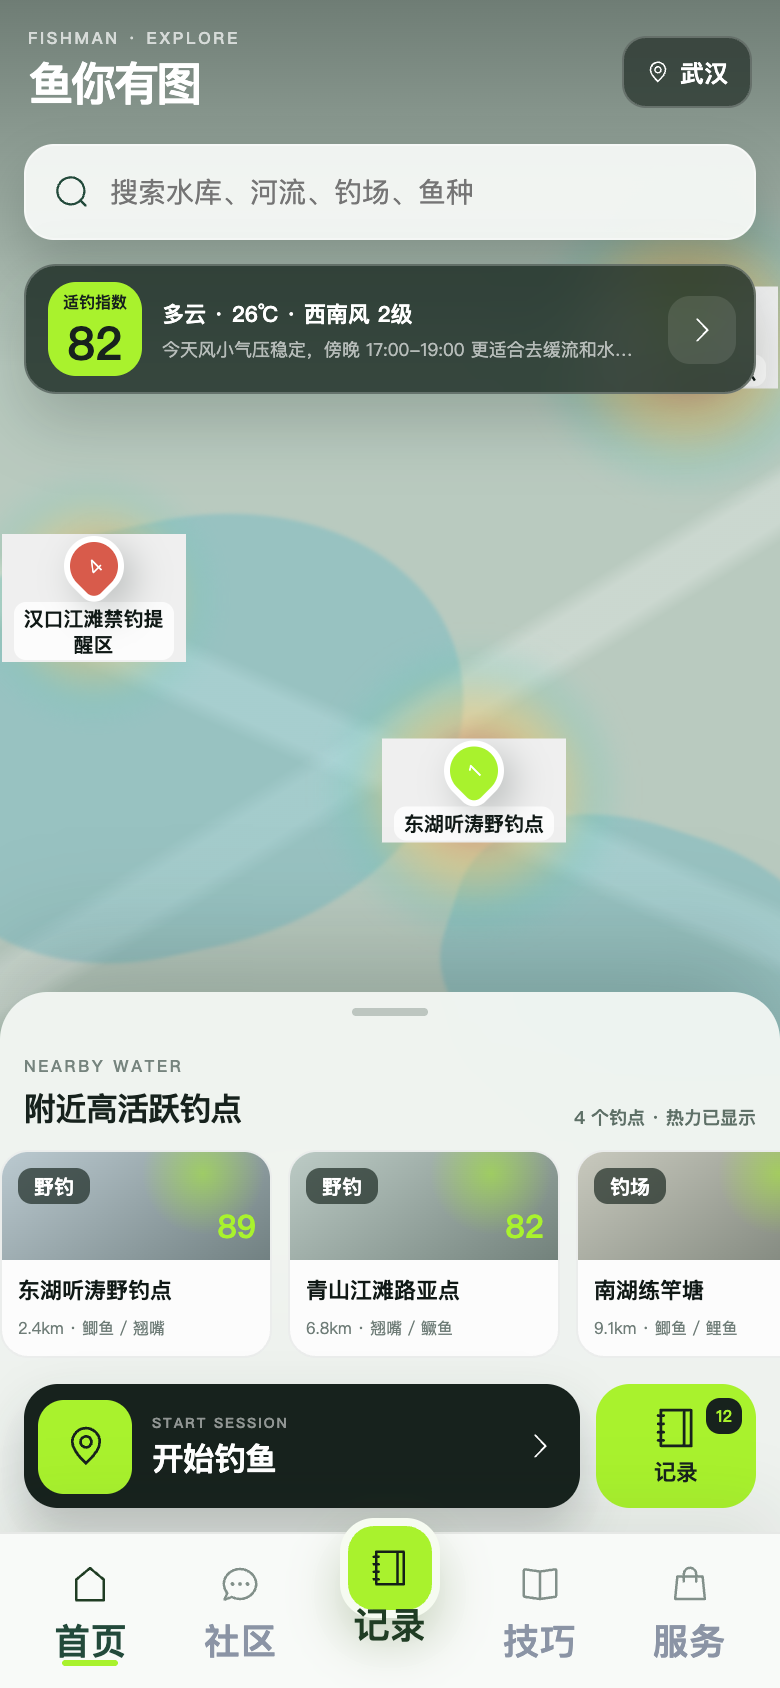
\includegraphics[height=0.68\textheight]{figures/page_home.png}
  \caption{首页截图（示例）}
  \label{fig:appendix-page-home}
\end{figure}


\end{document}
